\section{Cliques, ensembles indépendants et l'impossible désordre}

\subsection{Ensembles indépendants}

\begin{mytheo} [Théorème de l'amitié 1] \label{ami1}
  Parmi six personnes, on en trouve toujours trois qui se connaissent l'une l'autre, ou trois qui sont étrangers l'un à l'autre.
  \begin{proof}
     Considérons le graphe complet $K_6$ pour représenter le problème. Les nœuds symbolisent les personnes et les arêtes symbolisent les relations entre elles. Deux personnes sont reliées par une arêtes bleue si elles se connaissent, et par une arête rouge sinon. On veut montrer que le graphe contient un triangle bleu ou un triangle rouge.
     
     Chaque nœud $x$ a cinq voisins. On peut donc définir une couleur majoritaire en chaque nœud comme la couleur du plus grand nombre d'arêtes incidentes. Prenons le cas où la couleur majoritaire pour $x$ est le bleu. Il existe donc au moins trois arêtes bleues incidentes à $x$.
     
   \begin{figure} [!h]
   \centering
        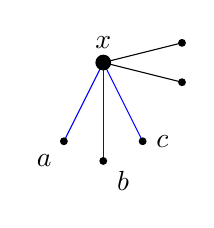
\begin{tikzpicture}[scale = 0.5]
                   \draw[blue] (0,1) -- (-1,-1);
                   \draw[blue] (0,1) -- (0,-1.5);
                   \draw[blue] (0,1) -- (1,-1);
                   \draw[black] (0,1) -- (2,0.5);
                   \draw[black] (0,1) -- (2,1.5);
                   
                   \fill[black] (0,1) circle (0.2cm);
                   \fill[black] (-1,-1) circle (0.1cm);
                   \fill[black] (0,-1.5) circle (0.1cm);
                   \fill[black] (1,-1) circle (0.1cm);
                   \fill[black] (2,0.5) circle (0.1cm);
                   \fill[black] (2,1.5) circle (0.1cm);
                   
                   \node at (0,1.5) {$x$};
                   \node at (-1.5,-1.5) {$a$};
                   \node at (0.5,-2) {$b$};
                   \node at (1.5,-1) {$c$};
                   
        \end{tikzpicture}             
	\end{figure}
     
     Considérons trois nœuds $a$, $b$ et $c$ reliés à $x$ par une arête bleue. Si ces trois nœuds forment un triangle rouge, alors le graphe contient un triangle rouge. Sinon, le triangle $abc$ contient au moins une arête bleue. Prenons par exemple l'arête $ab$ bleue. Le triangle $abx$ est alors bleu. Le graphe contient donc dans ce cas-ci un triangle bleu. 
     
     La preuve reste évidemment valable si l'on prend l'arête $bc$ ou l'arête $ac$ bleue, de même que si l'on prend le rouge comme couleur majoritaire du nœud $x$.
  \end{proof}
\end{mytheo}

\begin{mytheo} [Théorème de l'amitié 2] \label{ami2}
  En coloriant, de façon arbitraire, les arêtes du graphe complet à six nœuds en bleu et rouge, on crée un triangle bleu ou un triangle rouge.
  \begin{proof}
  	Voir théorème \ref{ami1}.
  \end{proof}
\end{mytheo}

\index{ensemble indépendant}
\begin{mydef}
  Un \emph{ensemble indépendant} d'un graphe est un ensemble de nœuds deux à deux non adjacents.
\end{mydef}

\index{ensemble indépendant!maximum}
\begin{mydef}
  Un \emph{ensemble indépendant maximum} est un ensemble indépendant dont le nombre de nœuds est maximal.
\end{mydef}

\begin{mytheo}
Un ensemble de nœuds est indépendant si et seulement si son complémentaire est une couverture de sommets.
\begin{proof}
Soit S un ensemble de nœuds indépendant.
 
S est un ensemble de nœuds indépendant. \\
$\Leftrightarrow$ Il n'existe pas d'arête rejoignant 2 nœuds de S. \\
$\Leftrightarrow$ Toute arête a au moins une extrémité qui n'est pas incluse dans S. \\
$\Leftrightarrow$ Le complémentaire de S est une couverture de sommets.
\end{proof}
\end{mytheo}

\begin{myexem} \label{cm7:ex1}
	Complémentaire d'un ensemble indépendant
	\begin{figure} [!h]
	\centering
         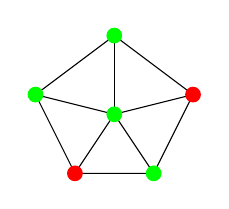
\begin{tikzpicture}[scale = 0.5]
             	   \draw (-1,0) -- (-2,2) -- (0,3.5) -- (2,2) -- (1,0) -- (-1,0) -- cycle;
                   \draw (-1,0) -- (0,1.5);
                   \draw (-2,2) -- (0,1.5);
                   \draw (0,3.5) -- (0,1.5);
                   \draw (2,2) -- (0,1.5);
                   \draw (1,0) -- (0,1.5);
                   
                   \fill[red] (-1,0) circle (0.2cm);
                   \fill[green] (-2,2) circle (0.2cm);
                   \fill[green] (0,3.5) circle (0.2cm);
                   \fill[red] (2,2) circle (0.2cm);
                   \fill[green] (1,0) circle (0.2cm);
                   \fill[green] (0,1.5) circle (0.2cm);
                   
        \end{tikzpicture}
	\end{figure} \newline
	\color{green}Couverture de sommets \\
	\color{red}Ensemble indépendant (maximal)
	\color{black}
\end{myexem}


\begin{mycorr} 
|ensemble indépendant maximum| + |couverture minimum| = |nombre de nœuds|
\end{mycorr}

Ainsi, trouver un ensemble indépendant maximum est tout aussi difficile que de trouver une couverture de sommets minimale.

\subsection{Cliques}

\begin{mydef}
Une \emph{clique} d'un graphe est un ensemble de nœuds deux à deux adjacents. Autrement dit, c'est un sous-graphe complet.
\end{mydef}

\index{clique!maximum}
\begin{mydef}
Une \emph{clique maximum} est une clique dont le nombre de nœuds est maximal.
\end{mydef}

\begin{mytheo}
  Un ensemble est indépendant dans un graphe simple si et seulement s'il est une clique dans le graphe complémentaire.
  \begin{proof}
     Soit S un ensemble indépendant dans un graphe simple G.
     
     S est un ensemble indépendant de G \\
     $\Leftrightarrow$ Deux nœuds quelconques de S sont non-adjacents dans G. \\
     $\Leftrightarrow$ Deux nœuds quelconques de S sont adjacents dans le complémentaire de G. \\
     $\Leftrightarrow$ S est une clique dans le complémentaire de G.\\
  \end{proof}
\end{mytheo}


\begin{myexem} Complémentaire du graphe de l'exemple \ref{cm7:ex1}
	\begin{figure} [!h]
	\centering
             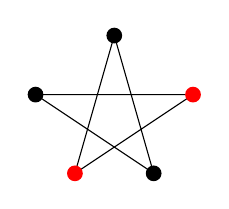
\begin{tikzpicture}[scale = 0.5]
                   \draw (-1,0) -- (0,3.5) -- (1,0) -- (-2,2) -- (2,2) -- (-1,0) -- cycle;
                   
                   \fill[red]   (-1,0)  circle (0.2cm);
                   \fill[black] (-2,2)  circle (0.2cm);
                   \fill[black] (0,3.5) circle (0.2cm);
                   \fill[red]   (2,2)   circle (0.2cm);
                   \fill[black] (1,0)   circle (0.2cm);
                   %\fill[black] (0,1.5) circle (0.2cm);
        \end{tikzpicture}
    \end{figure} \newline
    \color{red}Clique (maximum) \color{black}
\end{myexem}

\begin{mytheo} [Théorème de l'amitié 3]
  Tout graphe simple à six nœuds contient une clique de trois nœuds ou un ensemble indépendant de trois nœuds.
  \begin{proof}
     Soit $G$ un graphe simple. Si l'on colorie toutes les arêtes de $G$ en bleu et que l'on relie tous les nœuds non-adjacents de $G$ avec des arêtes rouges, par le théorème \ref{ami2}, il existe un triangle bleu ou un triangle rouge. On a donc montré qu'il existe une clique de trois nœuds (triangle bleu) ou un ensemble indépendant de trois nœuds (triangle rouge).
  \end{proof}
\end{mytheo}


\begin{mydef} [Nombre de Ramsey]
Le \emph{nombre de Ramsey} $R(n_1 , ..., n_k)$ est le plus petit naturel $r$ tel que tout coloriage du graphe complet de $r$ nœuds en $k$ couleurs $c_1$ , ..., $c_k$ crée une clique de $n_1$ nœuds de couleur $c_1$, ou une clique de $n_2$ nœuds de couleur $c_2$, ..., ou une clique de $n_k$ nœuds de couleur $c_k$.
\end{mydef}
  
\begin{mytheo} [Théorème de Ramsey]
Le nombre de Ramsey $R(n_1,...,n_k)$ existe.
\end{mytheo}

\begin{mytheo} [Théorème de Erdös et Szekeres]
  Pour $m, n \geq 2: R(m, n) \leq R(m, n-1) + R(m-1, n)$.
  \begin{proof}
     Prenons un noeud quelconque u dans un graphe complet à $R(m,n-1) + R(m-1,n)$ 
      avec des arêtes coloriées en bleu ou en rouge. Soit M et N définis tels que
     $$M = \{ \text{voisins de u reliés par des arêtes bleues}\}$$
     $$N = \{ \text{voisins de u reliés par des arêtes rouges}\}.$$
     
\begin{figure} [!h]
\centering
        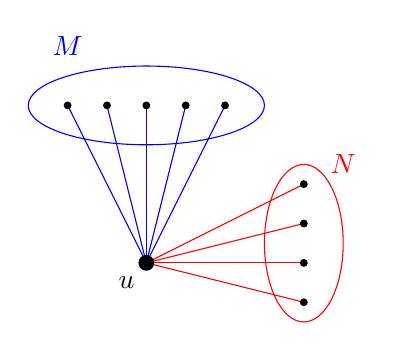
\begin{tikzpicture}[scale = 0.5]
                   \draw[blue] (-1,-2) -- (-3,2);
                   \draw[blue] (-1,-2) -- (-2,2);
                   \draw[blue] (-1,-2) -- (-1,2);
                   \draw[blue] (-1,-2) -- (0,2);
                   \draw[blue] (-1,-2) -- (1,2);
                   \draw[red] (-1,-2) -- (3,0);
                   \draw[red] (-1,-2) -- (3,-1);
                   \draw[red] (-1,-2) -- (3,-2);
                   \draw[red] (-1,-2) -- (3,-3);
                   
                   \fill[black] (-1,-2) circle (0.2cm);
                   \fill[black] (-3,2) circle (0.1cm);
                   \fill[black] (-2,2) circle (0.1cm);
                   \fill[black] (-1,2) circle (0.1cm);
                   \fill[black] (-0,2) circle (0.1cm);
                   \fill[black] ( 1,2) circle (0.1cm);
                   \fill[black] (3, 0) circle (0.1cm);
                   \fill[black] (3,-1) circle (0.1cm);
                   \fill[black] (3,-2) circle (0.1cm);
                   \fill[black] (3,-3) circle (0.1cm);
                   
                   \node at (-1.5,-2.5) {$u$};
                   \node at (-3,3.5) {\color{blue}$M$};
                   \node at (4,0.5) {\color{red}$N$};
                   
                   \draw[blue] (-1,2) ellipse (3cm and 1cm);
                   \draw[red]  (3,-1.5) ellipse (1cm and 2cm);                 
        \end{tikzpicture}          
\end{figure}   
     
 On a (simplement la somme des nœuds) que
 $$|M|+|N|+1 = R(m,n-1) + R(m-1,n).$$
 
 Donc on a que
 \begin{equation} \label{cm7:RM}
 |M| \geq R(m-1,n)
\end{equation}
ou bien
\begin{equation} \label{cm7:RN}
 |N| \geq R(m,n-1)
\end{equation}

Si on est dans le cas de figure de l'inégalité \ref{cm7:RM}, il y a deux possibilités. Soit il existe une clique rouge de $n$ nœuds dans $M$ ce qui implique qu'il existe une clique rouge de $n$ nœuds dans le graphe. Soit il existe une clique bleue de $m-1$ nœuds dans $M$ ce qui en incluant $u$ fait une clique bleue de $m$ nœuds dans le graphe.

Si on est dans le cas de figure de l'inégalité \ref{cm7:RN}, idem mutatis mutandis.
  \end{proof}
\end{mytheo}

\begin{mycorr} R(m,n) $\leq \begin{pmatrix}
m+n-2\\
m-1
\end{pmatrix}$\\
\end{mycorr}

\begin{mytheo}
$R(n_1,...,n_k) \leq R \left( n_1,...,n_{k-2},R(n_{k-1},n_k) \right)$

\begin{proof}
  Prenons un graphe complet à $R(n_1, ..., n_{k-2}, R(n_{k-1}, n_k))$ nœuds et leurs arêtes coloriées en $k$ couleurs. Soit $c_i $ la couleur $i$.
  
  Faisons semblant que $c_{k-1}$ et $c_{k}$ sont une seule couleur. Cela implique qu'il n'y a plus que $k-1$ couleurs. Il existe donc une clique à $n_1$ nœuds de couleur $c_1$ ou bien une clique à $n_2$ nœuds de couleur $c_2$ et ainsi de suite jusqu'à la possibilité d'une clique de $R(n_{k-1}, n_k)$ nœuds de couleur $c_{k-1}$ ou $c_{k}$.
  
  Or par définition de $R(n_{k-1}, n_k)$, cette dernière possibilité revient à dire qu'il existe une clique de $n_{k-1}$ nœuds de couleur $c_{k-1}$ ou une clique de $n_{k}$ nœuds de couleur $c_{k}$.
\end{proof}
\end{mytheo}

\vspace{0.3cm}
En d'autre termes, ce théorème stipule qu'il existe toujours un peu d'ordre dans un ensemble suffisamment grand.

\begin{mytheo} [Théorème de l'amitié 4]
  $R(3, 3) = 6$
  \begin{proof}
     Cela découle directement du théorème \ref{ami2}.
  \end{proof}
\end{mytheo}  
      

\begin{mytheo} 
[Théorème de Turán
\footnote{par la contraposée on obtient la définition de Wikipédia qui nous dit: Tout graphe $G$ ayant $n$ sommets, et ne contenant pas de clique de taille plus grande que $r$ ($ K_{r+1} $) possède au plus $(1-\frac{1}{r})\frac{n^2}{2}$ arêtes}] \label{turan}
Si un graphe simple possède strictement plus de $(1-\frac{1}{r})\frac{n^2}{2}$ arêtes, alors il a une clique de $n+1$ nœuds.
\end{mytheo}

Cette borne est atteinte par le graphe de Turán $T(n,r)$.  Selon wiki un graphe de $T(n,r)$ n'a pas de clique de taille $ r+1$ mais je ne sais pas si il existe un graphe $T(n,r)$ pour tout $r$.


\textbf{Notes :}
\begin{enumerate}
\item
Pendant les séances d'exercices, le tuteur a complété le théorème \ref{turan} en ajoutant "et il existe un graphe possédant $\left( 1-\dfrac{1}{r} \right) \dfrac{n^2}{2}$ qui ne contient aucune clique de taille $r+1$" (ce que Wikipédia semble confirmer).
\item
On a  $\left( 1-\dfrac{1}{n} \right) \dfrac{n^2}{2} > \left( 1-\dfrac{1}{n-1} \right) \dfrac{n^2}{2}$ donc si on prend $r=n$ alors on aura une clique à $(n-1)+1=n$ nœuds. Or on a bien : $\left( 1-\dfrac{1}{n} \right) \dfrac{n^2}{2} = \dfrac{n(n-1)}{2}$.
\end{enumerate}
   

\subsection{La théorie de Ramsey}
Beaucoup de théorèmes existent qui imitent le théorème de Ramsey et prouvent quelque chose du genre:
\begin{itemize}
\item
"Dans un machin suffisamment grand, il y a toujours des sous-machins avec une certaine propriété."
\item
"Dans un grand machin, m\^eme tout-à-fait quelconque, un certain ordre est inévitable."
\item
"Le désordre complet est impossible."
\end{itemize}
    
    
    
\begin{mytheo} [Sommes d'entiers]
    Si l'on colorie les nombres de un à quatorze en trois couleurs alors il existe trois nombres (pas forcément distincts) $x$, $y$ et $z$ de m\^eme couleur tels que $x+y=z$.
\end{mytheo}
 
\begin{myexem}   
Séparons les nombres de 1 à 13 en trois couleurs:
\vspace*{0.2cm}
    
    \begin{tabular}{|c|c|c|c|c|c|c|c|c|c|c|c|c|c|}
        \hline
       couleur1 & 1 &  &  & 4  &  &  &  &  &  & 10 &  &  & 13\\
       
       \hline
       couleur2 &  & 2 & 3 &  &  &  &  &  &  &  & 11 & 12 &\\
       
       \hline
       couleur3 &  &  &  &  & 5 & 6 & 7 & 8 & 9 &  &  &  &\\
  
        \hline
      \end{tabular} \\
      Le 14 ne va nulle part.
\end{myexem}

%\vspace*{0.2cm}
      
\begin{mytheo} [Théorème de Schur] 
Pour chaque $k$, il y a un nombre $r_k$ tel que pour toute partition des nombres $1,2,....,r_k$ en $k$ classes, une de ces classes contient $x$, $y$ et $z$ tels que $x+y=z$. \footnote{dans l'exemple ci-dessus $k = 3$ et $r_k = 14$}
\begin{proof}
Soit $r_k = R(n_1,...,n_k)$ avec $\forall i \in [1 , k], n_i = 3 $.

Colorions les ar\^etes du graphe à $r_k$ nœuds, sachant qu'on a réparti arbitrairement ses nœuds dans les classes $S_1 ,S_2,....,S_k$.

Nous allons les colorier de la manière suivante: l'ar\^ete $ij$ est dans la couleur $c$ si $\mid i-j \mid \in S_c $.\footnote{à priori il n'y a pas de raison particulière pour le choix "couleur $c$ si $\mid i-j \mid \in S_c $" mais ça fonctionne.} Nous utilisons donc $k$ couleurs différentes pour les arêtes.

Par le théorème de Ramsey, il y a un triangle monochrome.
Donc il y a $i$, $j$ et $l$ tels que:
\begin{itemize}
\item
$i < j < l$
\item
$j-i, l-j, l-i$ sont dans le m\^eme classe.\\      
\end{itemize}
      
On prend alors:\\
$x = j-i$, $y = l-j$ et $z = l-i$\\
$\Rightarrow x+y=z$

\end{proof}
\end{mytheo}


\begin{mytheo} [Théorème d'Esther Klein]
Parmi cinq points arbitraires dans le plan, tels que trois d'entre eux ne sont  jamais alignés, on peut toujours en choisir quatre qui déterminent un quadrilatère convexe.
\end{mytheo}

\begin{mytheo}
Si l'on colorie les nombres de un à neuf en deux couleurs.  Alors il existe une progression arithmétique de longueur trois qui est monochrome.
\end{mytheo}
     
\begin{mytheo} [Théorème de Van der Waerden]
Pour tout $k$, $l$, il existe un nombre $W(k,l)$ tel que les nombres de 1 à $W(k,l)$, coloriés arbitrairement en $k$ couleurs, contiennent une progression arithmétique monochrome de longueur $l$.
\end{mytheo}

\begin{myexem} Cherchons $W(2,3)$ expérimentalement.

\color{green}1 \color{green}2 \color{red}3 \color{green}4 \color{green}5  \color{red}6 \color{red}7 \color{black}8

On ne sait pas en quelle couleur colorier le huit car si on le met en rouge on crée la suite arithmétique 6, 7, 8, de raison un et en vert la suite 2, 5, 8, de raison 3.
\end{myexem}
